\chapter{Introdução}

  O tema do nosso trabalho é a análise de tendências no \nonport{YouTube}, com foco em compreender quais tipos de vídeos estão \emph{Em Alta} na plataforma, identificar os canais mais influentes e observar o engajamento que esses vídeos recebem, medido em termos de curtidas, comentários e visualizações. Através dessa análise, buscamos extrair \nonport{insights} que permitam caracterizar o que define um vídeo popular, os padrões de conteúdo que se destacam, e a relação entre a popularidade e o país de origem dos vídeos. Para isso, estamos nos guiando através das seguintes principais questões: ``Quais categorias de vídeos estão \emph{em alta}?'', ``Quais tipos de canais produzem o conteúdo mais relevante e visualizado?'', ``Como as tendências variam de acordo com as regiões?'' e ``Qual a relação entre quantidade de comentários e \nonport{likes} e a classificação de um vídeo?''. Essas perguntas, além de norteadoras, nos motivaram a escolher esse tema. Por meio desta análise, buscamos não apenas identificar padrões regionais e globais, mas também entender como os algoritmos da plataforma podem influenciar o comportamento do público e o sucesso de certos tipos de conteúdo.

  Consultas realizadas, assim como a modelagem física em \nonport{SQL}, a modelagem conceitual e lógica utilizando o \textit{brModelo}, e o \textit{data scraping} implementado em Python, podem ser encontrados em \cite{our-YoutubeScraperDataBank}.

\chapter{Datasets}

  Os conjuntos de dados utilizados estão sendo extraídos por meio de um programa em \var{python} --- que estamos chamando de \var{scraper} --- que na verdade é o \href{https://github.com/mitchelljy/Trending-YouTube-Scraper}{\var{YouTube Data Scraper} do usuário \var{mitchelljy}} em seu \href{https://github.com/mitchelljy}{\nonport{GitHub}} incrementado com diversas modificações que nos permitem extrair dados públicos de nosso interesse. A chave \href{https://developers.google.com/youtube/v3/docs?hl=pt-br}{\var{YouTube Data API v3}} que está sendo utilizada foi adquirida por meio do \nonport{YouTube} em uma de nossas próprias contas. Os dados extraídos pelo \var{scraper} são armazenados em um arquivos \nonport{CSV} que o próprio programa gera. Importante mencionar que a página do \var{mitchelljy} do \nonport{GitHub} foi encontrada por meio do site \nonport{Kaggle}\cite{kaggle}.

  Os dados contidos no \nonport{CSV} e seus respectivos tipos são:

  \begin{itemize}
    \item \var{video\underline{ }id}: contém, em cada registro, o \var{ID} do vídeo gerado pelo próprio \nonport{YouTube}. Esse \var{ID} é utilizado para, além de mera caracterização de vídeos únicos na plataforma, a geração de suas \textit{URL}s, por exemplo. Cada \var{ID} é uma sequência alfanumérica de símbolos, sendo mais apropriado modelá-lo como cadeia de caracteres (\nonport{string}) em nosso sistema;
    \item \var{title}: refere-se ao título do vídeo em sua língua original (em que foi publicado). Suporta caracteres de \nonport{UTF-8}. É, naturalmente, do tipo textual, sendo, portanto, claramente representável por valores do domínio de \nonport{strings};
    \item \var{publishedAt}: corresponde à data e hora de publicação do vídeo (com relação ao Tempo Universal Coordenado \nonport{UTC}). O valores desse atributo são resgatados no formato \href{https://www.w3.org/TR/NOTE-datetime}{\nonport{ISO 8601}} e podem ser mapeados para o domínio \nonport{DATETIME} do \nonport{SGBD};
    \item \var{channelId}: análogo ao \var{ID} gerado para o vídeo, este campo armazena o \var{ID} criado pelo site para cada canal, neste caso, o canal que publicou o vídeo. É uma cadeia alfanumérica e, consequentemente, está no domínio de \nonport{strings};
    \item \var{channelTitle}: também análogo ao título do vídeo, é relativo ao título do canal que postou o determinado vídeo. É do tipo textual e mapeado no tipo \nonport{string};
    \item \var{categoryId}: corresponde ao identificador da categoria atribuída ao vídeo pelo canal que o publicou. No \href{https://developers.google.com/youtube/v3/docs/videos?hl=pt-br#snippet.categoryId}{guia de referências da \nonport{API}} consta que é um dado do tipo \nonport{string}, porém, após coleta da listagem de categorias disponíveis, percebemos que todas se tratam de inteiros de 1 a 44 (pulando alguns). Portanto, consideramos que a atribuição ao domínio dos inteiros seja a melhor alternativa;
    \item \var{trending\underline{ }date}: contém a data em que o vídeo está \emph{em alta}, ou seja, equivale à data em que o arquivo \nonport{CSV} foi criado. Está em um formato diferente do utilizado pela \nonport{API} do \nonport{YouTube}, pois é uma informação adicionada artificialmente no \nonport{script}. Consiste do ano, dia e mês de coleta dos dados, nesta ordem, separados por ponto final (AA.DD.MM). É naturalmente associável ao domínio \nonport{DATE};
    \item \var{tags}: corresponde a uma lista de \nonport{tags} (etiquetas) atribuídas ao vídeo, usadas como auxílio para o algoritmo de recomendações da plataforma. São pequenas porções de texto (ocorrências de \var{tag}) separadas por vírgulas (`,'). É permitido que a \var{tag} contenha espaços. Cada \var{tag} encaixa-se no domínio string;
    \item \var{view\underline{ }count}: é o número total de visualizações que o vídeo teve desde sua publicação até o instante da captura dos dados. Consiste de um inteiro não-negativo (logicamente) e, por isso, pode ser modelado por um inteiro longo sem sinal;
    \item \var{likes}: é uma métrica numérica, assim como a contagem de visualizações, referente ao número de curtidas (\nonport{likes}) que o vídeo obteve até a coleta dos dados. É inteiro longo maior ou igual a zero;
    \item \var{comment\underline{ }count}: novamente, é um campo numérico que retrata a quantidade de comentários que o vídeo recebeu até a captura dos dados. Pertence ao domínio de inteiros longos sem sinal;
    \item \var{thumbnail\underline{ }link}: é a \nonport{URL} da \nonport{thumbnail} (imagem de capa) do vídeo. Por ser um \nonport{link}, que é composto por vários caracteres, alfanuméricos e símbolos especiais, em sequência, escolhemos o tipo \nonport{string} para armazená-los;
    \item \var{comments\underline{ }disabled}: indica se o canal que publicou o vídeo optou por desativar a postagem de comentários. Nos arquivos \nonport{CSV}, esse campo é assinalado por \var{True} ou \var{False}, devendo, evidentemente, ser tratado como um valor de domínio \nonport{booleano};
    \item \var{ratings\underline{ }disabled}: informa se o canal desativou a opção dos espectadores curtirem (ou descurtirem) o vídeo. Assim como \var{comments\underline{ }disabled}, somente assume valores \var{True} e \var{False} e, por isso, é traduzido para valores do espectro \nonport{booleano};
    \item \var{description}: é a \href{https://developers.google.com/youtube/v3/docs/videos?hl=pt-br#snippet.description}{descrição} do vídeo fornecida pelo seu publicador na língua original. É um texto de tamanho completamente variável (no máximo 5000 caracteres) e pode conter símbolos da codificação \nonport{UTF-8}. Logo, é do tipo \nonport{string}.
    \item \var{channel\underline{ }creation\underline{ }date}: diz respeito à data e hora (no mesmo formato \var{ISO 8601} do campo \var{published\underline{ }at}) de criação do canal que publicou o vídeo. É mapeado no domínio \nonport{DATETIME} do \var{SGBD};
    \item \var{channel\underline{ }subscriber\underline{ }count}: corresponde ao número de inscritos que o canal publicador possui no momento da coleta de dados. Assim como as métricas do vídeo, é um dado altamente mutável e que assume valores inteiros potencialmente grandes. Por esse motivo, optamos por usar o domínio \nonport{BIGINT};
    \item \var{channel\underline{ }video\underline{ }count}: é a quantidade de vídeos publicados, até então, pelo canal responsável pelo vídeo em questão. Dificilmente passará a marca de $2^{31} - 1$, então assumimos tipo inteiro de $4$ \nonport{bytes};
    \item \var{video\underline{ }url}: condiz com a URL gerada pelo YouTube para o vídeo (que foi discutida na descrição de \var{video\underline{ }id}). É obtida, no código de coleta e organização dos dados, a partir da concatenação da URL padrão para redirecionamento em vídeo com o \var{ID} do vídeo. Por corresponder a uma sequência de caracteres, é melhor modelado por uma string;
    \item \var{channel\underline{ }description}: refere-se a uma descrição textual do canal dada por seu criador, similar à descrição do vídeo. Escolheu-se o tipo \nonport{TEXT} para armazená-la do banco de dados;
    \item \var{channel\underline{ }image}: relativo ao ícone do canal. Seu formato é de uma URL que redireciona para a imagem em questão. Por isso, decidimos tratar como \nonport{string};
    \item \var{channel\underline{ }country}: configura o código do país ao qual o canal publicador está associado. É determinado por uma \nonport{string} de exatamente dois caracteres (ou três para \var{N/A}, se o canal não o possui) e \emph{supomos} que equivale ao padrão \href{https://www.iso.org/iso-3166-country-codes.html}{\var{ISO 3166-1}}\cite{iso-3166}

    (não encontramos evidências explícitas sobre isso na \href{https://developers.google.com/youtube/v3/docs/channels?hl=pt-br#snippet.country}{documentação da API}, apenas conferimos por inspeção). Portanto, é uma \nonport{string} de tamanho máximo 3;

    \item \var{channel\underline{ }total\underline{ }views}: relacionado com a quantidade total de visualizações que o canal teve em toda sua história. Como considerável parte dos canais listados dentre os vídeos \emph{em alta} são de alta relevância, os valores nesse campo são bem grandes e só conseguem ser armazenados se tratados como inteiros longos;
    \item \var{channel\underline{ }keywords}: é uma lista de palavras-chave escolhidas pelo detentor do canal para facilitar o trabalho de algoritmos de recomendação (assim como as tags dos vídeos). No conjunto de dados gerado, corresponde a uma grande \nonport{string} com as palavras-chave sendo separadas por espaços (` '). Cada palavra-chave é uma \nonport{string} e todas, juntas, \href{https://developers.google.com/youtube/v3/docs/channels?hl=pt-br#brandingSettings.channel.keywords}{podem somar até 500 caracteres}\cite{google_youtube_channels};
    \item \var{channel\underline{ }url}: trata-se da URL padrão do canal que postou o vídeo, aquela que o próprio YouTube gera através da concatenação do ID do canal ao esquema genérico de um link para canal (foi exatamente dessa forma que foi modelado no script que fornece o dataset). Guardamos cada valor desse campo em uma \nonport{string}.




  \end{itemize}

\chapter{Projeto do Banco de Dados}

\section{Modelo Conceitual}

  \vspace{2cm}
  \begin{figure}[H]
    \centering
    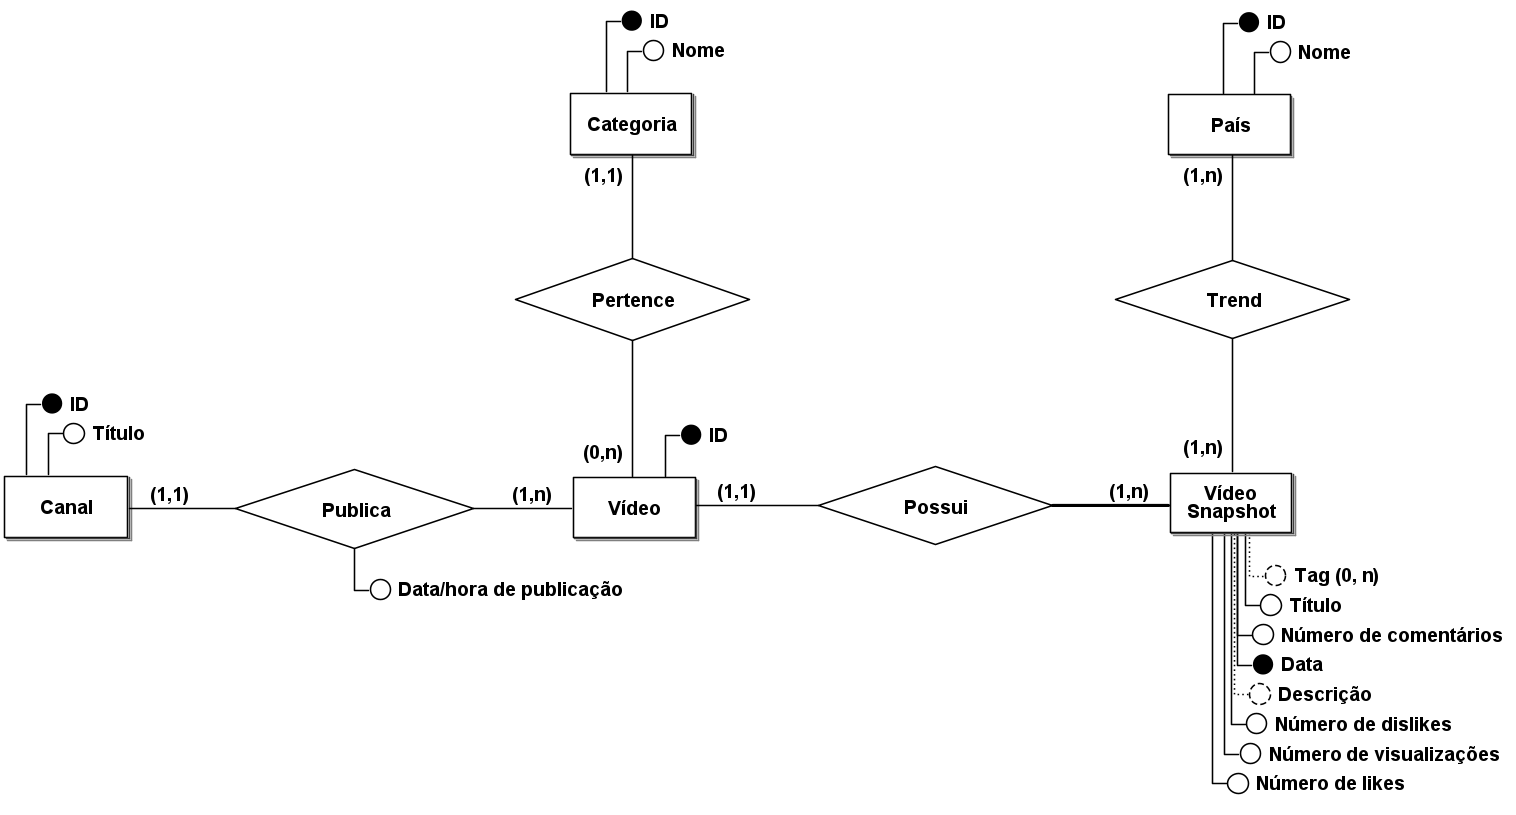
\includegraphics[width=1.0\linewidth]{conceitual.png}
    \caption{Modelagem Conceitual do \nonport{Dataset} utilizado.}
  \end{figure}

  \todo{Gustavo: Nessa seção, não discutimos a entidade Vídeo, sem Snapshot, em momento algum}

  O foco da nossa modelagem está em capturar o estado temporal de canais e vídeos \emph{em alta}. As entidades principais são o \var{Canal Snapshot} e o \var{Vídeo Snapshot}, que representam ``fotografias'' do estado de um canal e de um vídeo em um momento específico.

  O \var{Canal Snapshot} armazena informações temporais sobre um canal, como número de visualizações, inscritos, palavras-chave, título, número de vídeos, data da \nonport{snapshot}, \nonport{link}, descrição e imagem de perfil. Cada \var{Canal Snapshot} está associado a um \var{País}, o que permite registrar as características do canal em um contexto geográfico específico. Essa abordagem nos permite acompanhar a evolução e a presença do canal em diferentes regiões ao longo do tempo.

  Por outro lado, a entidade \var{Vídeo Snapshot} captura o estado de um vídeo em uma data específica, incluindo atributos como título, número de comentários, data, descrição, número de visualizações e número de likes. Essa estrutura é essencial para registrar a popularidade do vídeo exclusivamente na data em que ele se torna viral ou aparece no \emph{Em Alta}. A entidade \var{Trend} conecta cada \var{Vídeo Snapshot} a um \var{País}, representando os momentos em que o vídeo esteve em destaque em uma região específica, possibilitando uma análise detalhada de sua trajetória de popularidade.

  Além disso, a modelagem inclui a entidade \var{Canal}, que representa o canal original que publica os vídeos e possui atributos fixos, como ID e data de criação. Cada vídeo é publicado por um canal e é classificado em uma \var{Categoria} (como \var{Gaming} ou \var{Comedy}, por exemplo), que permanece inalterada ao longo do tempo.

  Essa modelagem com \var{Canal Snapshot} e \var{Vídeo Snapshot} como entidades centrais possibilita o monitoramento detalhado dos vídeos \emph{em alta}, permitindo acompanhar seus atributos em diferentes períodos e regiões.

  Além disso, colocamos uma observação na modelagem que \var{``Data'' em ``Canal Snapshot'' se e somente se ``Data'' em ``Video Snapshot''}. Tivemos que colocar essa restrição visto que nossa extração de dados garante que sempre que haja uma instância de \var{Canal Snapshot} com determinada \var{Data}, necessariamente há uma instância de \var{Vídeo Snapshot} com mesma \var{Data} e, analogamente, sempre que haja uma instância de \var{Vídeo Snapshot} com determinada \var{Data}, necessariamente há uma instância de \var{Canal Snapshot} com mesma \var{Data}.


\newpage
\section{Modelo Lógico}

  \vspace{2cm}
  \begin{figure}[H]
    \centering
    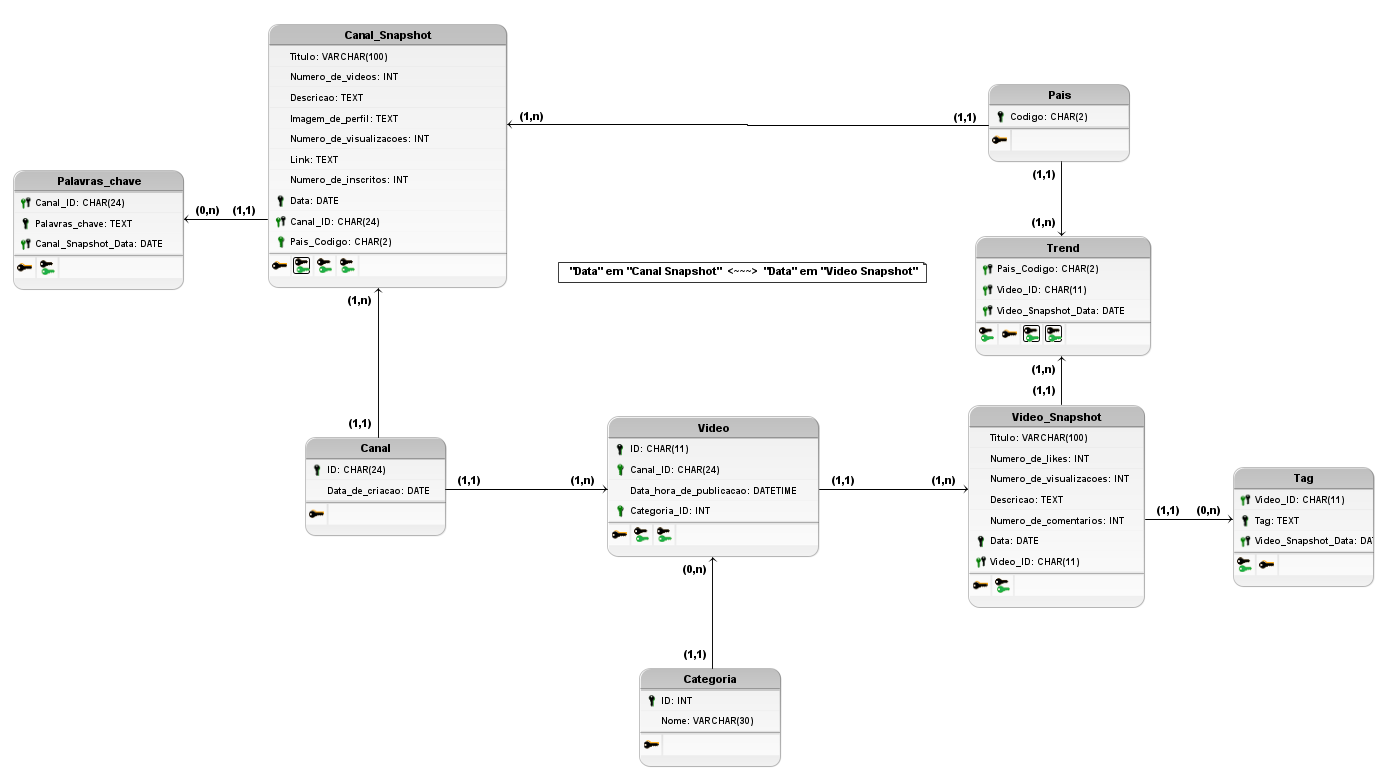
\includegraphics[width=1.0\linewidth]{logico.png}
    \caption{Modelagem Lógica do \nonport{Dataset} utilizado.}
  \end{figure}

  \todo{(Gustavo) Padronizar o uso de letras maiúsculas (ou minúsculas) no nome do brModelo/BRModelo ao longo do documento}

  Utilizamos a própria ferramenta \var{BRModelo} para a tradução da modelagem conceitual para a modelagem lógica. Ainda assim, o resultado da tradução apresentou diversos erros como chaves primárias e estrangeiras em locais errados, nomes de variáveis incoerentes. Sendo assim, tivemos que corrigir esses detalhes da modelagem lógica gerada pela ferramenta.

  Acreditamos que, após nossas correções, o modelo lógico representa nosso modelo com exatidão.

\newpage
\section{Modelo Físico}
\subsection{Criação da Modelagem}

Primeiramente, a modelagem física foi projetada diretamente da lógica, da qual convertemos para a física utilizando a ferramenta presente no próprio brModelo, fazendo as alterações necessárias conforme fomos verificando os erros da conversão automática. Após isso, para popular o banco de dados, utilizamos o \nonport{CSV} gerado pela \textit{API}, separando-o em outros \nonport{CSV}s menores que correspondiam a cada tabela (utilizando a biblioteca \var{pandas} da linguagem \var{Python} para tratar o formato dos dados e fazer essa separação), portanto, continham apenas as colunas requeridas por cada uma. Dito isso, foi utilizada uma função de importação, do próprio \var{SQL}, que importa todas as linhas de um \nonport{CSV} para tuplas de uma tabela específica. A seguir, encontra-se o código utilizado para a criação dos esquemas desse banco de dados e como os populamos com os \nonport{CSV}s gerados (junto com o código de criação).

\begin{enumerate}
  \item Tabela \var{Video}

  \begin{code}
    CREATE TABLE Video (
      ID CHAR(11) PRIMARY KEY,
      Canal_ID CHAR(24),
      Data_hora_de_publicacao DATE,
      Categoria_ID INT
    );
  \end{code}

  A tabela \var{Video} contém informações de cada vídeo, incluindo um identificador único, um campo de identificação para o canal responsável, a data de publicação e a categoria do vídeo.

  \item Tabela \var{Categoria}

  \begin{code}
    CREATE TABLE Categoria (
      ID INT PRIMARY KEY,
      Nome VARCHAR(30)
    );
  \end{code}

  A tabela \var{Categoria} armazena as categorias disponíveis, onde cada categoria possui um identificador e um nome. Essa tabela foi populada utilizando um \nonport{CSV} estático que contém todas as categorias possíveis.

  \item Tabela \var{Canal}

  \begin{code}
    CREATE TABLE Canal (
      ID CHAR(24) PRIMARY KEY,
      Data_de_criacao DATE
    );
  \end{code}

  A tabela \var{Canal} define os canais existentes, identificados por um ID único e com uma data de criação.

  \item Tabela \var{Pais}

  \begin{code}
    CREATE TABLE Pais (
      Codigo VARCHAR(3) PRIMARY KEY
    );
  \end{code}

  A tabela \var{Pais} apenas registra os códigos dos países, onde seu código é a chave primária. Inicialmente, tivemos um problema ao converter os valores do \nonport{CSV} para essa tabela, causando comportamentos inesperados no código. Por algum motivo, os campos do \nonport{CSV} não eram lidos com o tipo correto que era previsto, gerando diversos erros ao tentar adicionar chaves estrangeiras para essas tabelas, pois não estava havendo correspondência. Resolvemos, temporariamente, colocando os valores de forma manual nessa tabela.

  Foi necessário um tratamento adicional nos dados, pois, além de vários países duplicados, alguns canais não eram associados com nenhum país. Sendo assim, deixamos os canais sem países associados ao país \var{N/A} por padrão, porque estava havendo erros ao tentar utilizar a chave estrangeira com a tabela \var{Pais}, como já foi dito (e ao adicionar valores \var{NULL}).

  \item Tabela \var{Video\underline{ }Snapshot}

  \begin{code}
    CREATE TABLE Video_Snapshot (
      Titulo VARCHAR(100),
      Numero_de_likes BIGINT,
      Numero_de_visualizacoes BIGINT,
      Descricao TEXT,
      Numero_de_comentarios BIGINT,
      Data DATE,
      Video_ID CHAR(11),
      PRIMARY KEY (Data, Video_ID)
    );
  \end{code}

  A tabela \var{Video\underline{ }Snapshot} guarda informações em um certo momento do tempo detalhadas de cada vídeo, como o título, número de likes, visualizações, descrição, número de comentários e a data específica desse instante dos dados, vinculados ao vídeo identificado pelo \var{ID} do vídeo. Esta tabela permite o registro de \nonport{snapshots} dos dados de vídeos ao longo do tempo.

  \item Tabela \var{Canal\underline{ }Snapshot}

  \begin{code}
    CREATE TABLE Canal_Snapshot (
      Titulo VARCHAR(100),
      Numero_de_videos INT,
      Descricao TEXT,
      Imagem_de_perfil TEXT,
      Numero_de_visualizacoes BIGINT,
      Link TEXT,
      Numero_de_inscritos BIGINT,
      Data DATE,
      Canal_ID CHAR(24),
      Pais_Codigo VARCHAR(3),
      PRIMARY KEY (Data, Canal_ID)
    );
  \end{code}

  De maneira similar à anterior, a tabela \var{Canal\underline{ }Snapshot} armazena \nonport{snapshots} de canais de um certo momento no tempo, com dados sobre título, número de vídeos, descrição, imagem de perfil, visualizações totais, link, número de inscritos, a data da \nonport{snapshot} e o país do canal.

  Também foi necessário um tratamento adicional aqui, pois alguns canais aparecem mais de uma vez de maneira errônea.

  \item Tabela \var{Tag}

  \begin{code}
    CREATE TABLE Tag (
      Video_ID CHAR(11) NOT NULL,
      Tag VARCHAR(500),
      Video_Snapshot_Data DATE,
      PRIMARY KEY (Video_ID, Tag, Video_Snapshot_Data)
    );
  \end{code}

  A tabela \var{Tag} registra as \nonport{tags} associadas a cada vídeo, e cada linha possui o identificador do vídeo, uma lista das \nonport{tags} e a data do \nonport{snapshot} de vídeo relacionado, permitindo manter as \nonport{tags} de um vídeo em diferentes \nonport{snapshots}. (No código, foi utilizado uma função para lidar com esses campos multivalorados, separando em diversas linhas distintas).

  Nesse caso, tivemos que utilizar a função \var{explode} do pandas para separar campos multivalorados em diversas linhas

  \item Tabela \var{Palavra\underline{ }Chave}

  \begin{code}
    CREATE TABLE Palavra_chave (
      Canal_ID CHAR(24) NOT NULL,
      Palavra_chave VARCHAR(500),
      Canal_Snapshot_Data DATE,
      PRIMARY KEY (Canal_ID, Palavra_chave, Canal_Snapshot_Data)
    );
  \end{code}

  De modo equivalente, a tabela \var{Palavra\underline{ }chave} armazena palavras-chave de cada canal, relacionadas às datas das \nonport{snapshots} específicas do canal.

  Aqui, tivemos que usar novamente a função para separar um campo multivalorado em diversas outras linhas.

  \item Tabela \var{Trend}

  \begin{code}
    CREATE TABLE Trend (
      Pais_Codigo VARCHAR(3),
      Video_ID CHAR(11),
      Video_Snapshot_Data DATE,
      PRIMARY KEY (Pais_Codigo, Video_ID, Video_Snapshot_Data)
    );
  \end{code}

  Por fim, a tabela \var{Trend} contém informações sobre as tendências dos vídeos, associadas ao código do país, ao vídeo e ao snapshot de vídeo de uma data específica.
\end{enumerate}

Depois da declaração dos esquemas, foi feito a declaração das chaves estrangeiras de acordo com o planejado no modelo lógico, ficando:

\begin{code}
ALTER TABLE Video ADD CONSTRAINT FK_Video_Canal_ID
  FOREIGN KEY (Canal_ID)
  REFERENCES Canal (ID)
  ON DELETE RESTRICT;

ALTER TABLE Video ADD CONSTRAINT FK_Video_Categoria_ID
  FOREIGN KEY (Categoria_ID)
  REFERENCES Categoria (ID)
  ON DELETE RESTRICT;

ALTER TABLE Video_Snapshot ADD CONSTRAINT FK_Video_Snapshot_Video_ID
  FOREIGN KEY (Video_ID)
  REFERENCES Video (ID)
  ON DELETE CASCADE;

ALTER TABLE Canal_Snapshot ADD CONSTRAINT FK_Canal_Snapshot_Canal_ID
  FOREIGN KEY (Canal_ID)
  REFERENCES Canal (ID)
  ON DELETE CASCADE;

ALTER TABLE Canal_Snapshot ADD CONSTRAINT
  FK_Canal_Snapshot_Pais_Codigo
  FOREIGN KEY (Pais_Codigo)
  REFERENCES Pais (Codigo)
  ON DELETE RESTRICT;

ALTER TABLE Tag ADD CONSTRAINT FK_Tag_Video_ID
  FOREIGN KEY (Video_ID)
  REFERENCES Video_Snapshot (Video_ID)
  ON DELETE CASCADE;

ALTER TABLE Tag ADD CONSTRAINT FK_Tag_Video_Snapshot_Data
  FOREIGN KEY (Video_Snapshot_Data)
  REFERENCES Video_Snapshot (Data)
  ON DELETE CASCADE;

ALTER TABLE Palavra_chave ADD CONSTRAINT
  FK_Palavra_chave_Canal_Snapshot_Data
  FOREIGN KEY (Canal_Snapshot_Data)
  REFERENCES Canal_Snapshot (Data)
  ON DELETE CASCADE;

ALTER TABLE Palavra_chave ADD CONSTRAINT FK_Palavra_chave_Canal_ID
  FOREIGN KEY (Canal_ID)
  REFERENCES Canal_Snapshot (Canal_ID)
  ON DELETE CASCADE;

ALTER TABLE Trend ADD CONSTRAINT FK_Trend_Pais_Codigo
  FOREIGN KEY (Pais_Codigo)
  REFERENCES Pais (Codigo)
  ON DELETE RESTRICT;

ALTER TABLE Trend ADD CONSTRAINT FK_Trend_Video_ID
  FOREIGN KEY (Video_ID)
  REFERENCES Video_Snapshot (Video_ID)
  ON DELETE RESTRICT;

ALTER TABLE Trend ADD CONSTRAINT FK_Trend_Video_Snapshot_Data
  FOREIGN KEY (Video_Snapshot_Data)
  REFERENCES Video_Snapshot (Data)
  ON DELETE RESTRICT;
\end{code}

\subsection{Evidência de População do Banco de Dados}

Como evidência de criação e população do banco, segue capturas de telas das seguintes consultas:

\subsubsection{Canal}

\begin{figure}[H]
  \centering
  \begin{minipage}[b]{0.25\textwidth}
      \centering
      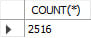
\includegraphics[width=\textwidth]{canal.jpg}
      \caption{Contador de \var{Canal}}
  \end{minipage}
  \hspace{0.05\textwidth}
  \begin{minipage}[b]{0.6\textwidth}
      \centering
      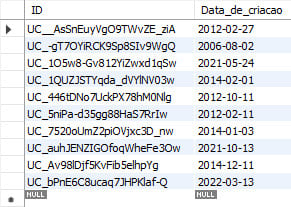
\includegraphics[width=\textwidth]{canal2.jpg}
      \caption{Exemplo de dados relativos a \var{canal}}
  \end{minipage}
\end{figure}

\subsubsection{Canal Snapshot}

\begin{figure}[H]
  \centering
  \begin{minipage}[b]{0.25\textwidth}
      \centering
      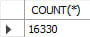
\includegraphics[width=\textwidth]{canal-snap.jpg}
      \caption{Contador de \var{Canal\underline{ }Snapshot}}
  \end{minipage}
  \hspace{0.05\textwidth}
  \begin{minipage}[b]{0.6\textwidth}
      \centering
      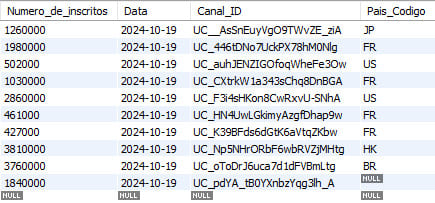
\includegraphics[width=\textwidth]{canal-snap3.jpg}
      \caption{Exemplo de dados relativos a \var{Canal\underline{ }Snapshot}}
  \end{minipage}
\end{figure}

\begin{figure}[H]
  \centering
  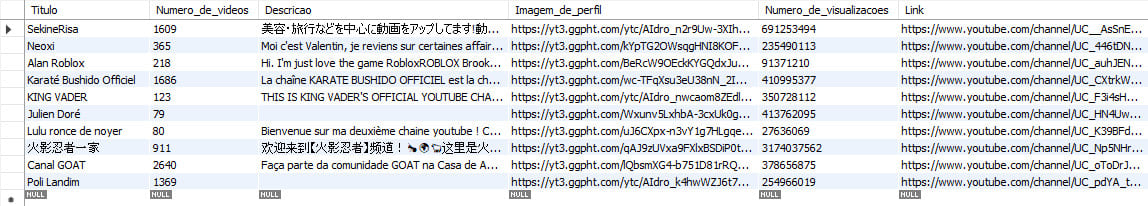
\includegraphics[width=\textwidth]{canal-snap2.jpg}
  \caption{Exemplo de dados relativos a \var{Canal\underline{ }Snapshot}}
\end{figure}

\subsubsection{Categoria}

\begin{figure}[H]
  \centering
  \begin{minipage}[b]{0.25\textwidth}
      \centering
      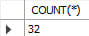
\includegraphics[width=\textwidth]{categorias.jpg}
      \caption{Contador de \var{Categoria}}
  \end{minipage}
  \hspace{0.05\textwidth}
  \begin{minipage}[b]{0.6\textwidth}
      \centering
      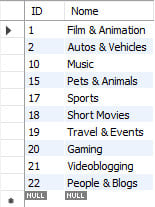
\includegraphics[width=0.4\textwidth]{categorias2.jpg}
      \caption{Exemplo de dados relativos a \var{Categoria}}
  \end{minipage}
\end{figure}

\subsubsection{Pais}

\begin{figure}[H]
  \centering
  \begin{minipage}[b]{0.25\textwidth}
      \centering
      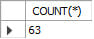
\includegraphics[width=\textwidth]{pais.jpg}
      \caption{Contador de \var{Pais}}
  \end{minipage}
  \hspace{0.05\textwidth}
  \begin{minipage}[b]{0.6\textwidth}
      \centering
      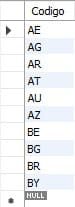
\includegraphics[width=0.2\textwidth]{pais2.jpg}
      \caption{Exemplo de dados relativos a \var{Pais}}
  \end{minipage}
\end{figure}

\subsubsection{Palavra Chave}

\begin{figure}[H]
  \centering
  \begin{minipage}[b]{0.25\textwidth}
      \centering
      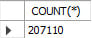
\includegraphics[width=\textwidth]{palavra-chave.jpg}
      \caption{Contador de \var{Palavra\underline{ }Chave}}
  \end{minipage}
  \hspace{0.05\textwidth}
  \begin{minipage}[b]{0.6\textwidth}
      \centering
      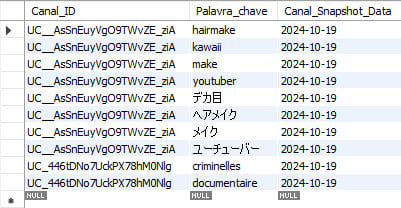
\includegraphics[width=\textwidth]{palavra-chave2.jpg}
      \caption{Exemplo de dados relativos a \var{Palavra\underline{ }Chave}}
  \end{minipage}
\end{figure}

\subsubsection{Tag}

\begin{figure}[H]
  \centering
  \begin{minipage}[b]{0.25\textwidth}
      \centering
      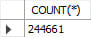
\includegraphics[width=\textwidth]{tag.jpg}
      \caption{Contador de \var{Tag}}
  \end{minipage}
  \hspace{0.05\textwidth}
  \begin{minipage}[b]{0.6\textwidth}
      \centering
      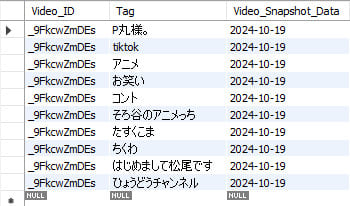
\includegraphics[width=\textwidth]{tag2.jpg}
      \caption{Exemplo de dados relativos a \var{Tag}}
  \end{minipage}
\end{figure}

\subsubsection{Trend}

\begin{figure}[H]
  \centering
  \begin{minipage}[b]{0.25\textwidth}
      \centering
      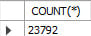
\includegraphics[width=\textwidth]{trend.jpg}
      \caption{Contador de \var{Trend}}
  \end{minipage}
  \hspace{0.05\textwidth}
  \begin{minipage}[b]{0.6\textwidth}
      \centering
      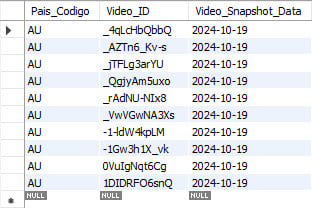
\includegraphics[width=\textwidth]{trend2.jpg}
      \caption{Exemplo de dados relativos a \var{Trend}}
  \end{minipage}
\end{figure}

\subsubsection{Video}

\begin{figure}[H]
  \centering
  \begin{minipage}[b]{0.25\textwidth}
      \centering
      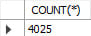
\includegraphics[width=\textwidth]{video.jpg}
      \caption{Contador de \var{Video}}
  \end{minipage}
  \hspace{0.05\textwidth}
  \begin{minipage}[b]{0.6\textwidth}
      \centering
      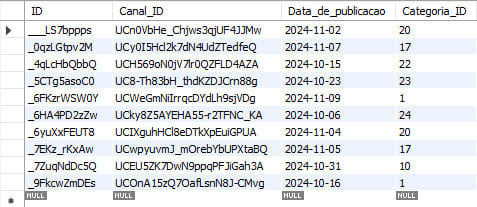
\includegraphics[width=\textwidth]{video2.jpg}
      \caption{Exemplo de dados relativos a \var{Video}}
  \end{minipage}
\end{figure}

\subsubsection{Video Snapshot}

\begin{figure}[H]
  \centering
  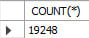
\includegraphics[width=0.25\textwidth]{video-snap.jpg}
  \caption{Contador de \var{Video\underline{ }Snapshot}}
\end{figure}

\begin{figure}[H]
  \centering
  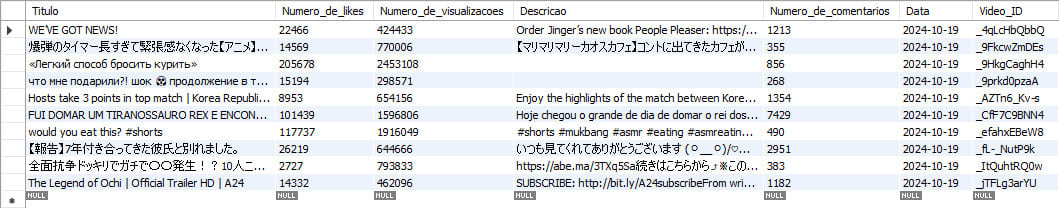
\includegraphics[width=\textwidth]{video-snap2.jpg}
  \caption{Exemplo de dados relativos a \var{Video\underline{ }Snapshot}}
\end{figure}
\section{Consultas}

\subsection{Views Auxiliares}

  Antes de realizarmos algumas consultas, decidimos por criar algumas \nonport{views} que nos auxiliassem, sendo elas:

  \begin{code}
-- VISOES AUXILIARES:

-- IDs dos videos e suas ultimas datas de aparicao no Em Alta de cada pais
CREATE VIEW Ultima_aparicao_video_pais AS
SELECT V.ID AS Video_ID, T.Pais_Codigo, MAX(VS.Data) AS Ultima_data
FROM Video AS V JOIN
    Video_Snapshot AS VS ON V.ID = VS.Video_ID JOIN
      Trend AS T ON V.ID = T.Video_ID AND
              VS.Data = T.Video_Snapshot_Data
GROUP BY V.ID, T.Pais_Codigo;

-- IDs dos videos e suas ultimas datas de aparicao no Em Alta
CREATE VIEW Ultima_aparicao_video AS
SELECT Video_ID, MAX(Ultima_Data) AS Ultima_data
FROM Ultima_aparicao_video_pais
GROUP BY Video_ID;

-- IDs dos canais e suas ultimas datas de aparicao no Em Alta de cada pais
CREATE VIEW Ultima_aparicao_canal_pais AS
SELECT C.ID AS Canal_ID, UAVP.Pais_Codigo, MAX(UAVP.Ultima_Data) AS Ultima_data
FROM Ultima_aparicao_video_pais AS UAVP JOIN
    Video AS V ON UAVP.Video_ID = V.ID JOIN
      Canal AS C ON V.Canal_ID = C.ID
GROUP BY C.ID, UAVP.Pais_Codigo;
  \end{code}

\subsection{Primeira consulta}

  Essa consulta exibe, em ordem decrescente, os canais que mais apareceram no \emph{Em Alta} e a quantidade de vezes que isso aconteceu. Consideramos como aparição cada ocorrência de um vídeo do canal no \emph{Em Alta} de um país em uma data.

\begin{code}
SELECT CS.Titulo AS Canal, COUNT(CS.Canal_ID) AS Numero_de_aparicoes
FROM Trend AS T JOIN
    Video_Snapshot AS VS ON T.Video_ID = VS.Video_ID AND
                T.Video_Snapshot_Data = VS.Data JOIN
      Video AS V ON VS.Video_ID = V.ID JOIN
        Canal AS C ON V.Canal_ID = C.ID JOIN
          Canal_Snapshot AS CS ON C.ID = CS.Canal_ID AND
                      VS.Data = CS.Data
GROUP BY CS.Titulo
ORDER BY Numero_de_aparicoes DESC;
\end{code}

\begin{figure}[H]
  \centering
  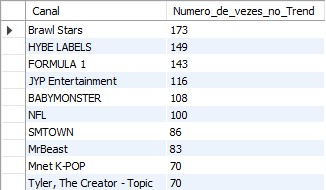
\includegraphics[width=0.5\textwidth]{consulta (1).jpg}
  \caption{Primeira consulta.}
\end{figure}

\subsection{Segunda consulta}

  A seguinte consulta exibe, em ordem decrescente, o número de vezes que uma tag apareceu em algum vídeo \emph{em alta}. Consideramos como aparição cada ocorrência de uma tag em um vídeo no \emph{Em Alta} de um país em uma data.

\begin{code}
SELECT Tag, COUNT(Tag) AS Numero_de_usos
FROM Ultima_aparicao_video_pais AS UAVP JOIN
    Tag AS T ON UAVP.Video_ID = T.Video_ID AND
          UAVP.Ultima_data = T.Video_Snapshot_Data
GROUP BY Tag
ORDER BY Numero_de_usos DESC;
\end{code}

\begin{figure}[H]
  \centering
  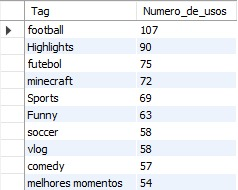
\includegraphics[width=0.4\textwidth]{consulta (2).jpg}
  \caption{Segunda consulta.}
\end{figure}

\subsection{Terceira consulta}

  Essa consulta exibe, em ordem decrescente, o número de vezes que uma palavra-chave apareceu em algum canal \emph{em alta}. Consideramos como aparição cada ocorrência de uma palavra-chave em um canal para cada vídeo seu no \emph{Em Alta} de um país em uma data.

\begin{code}
SELECT Palavra_chave, COUNT(Palavra_chave) AS Numero_de_usos
FROM Ultima_aparicao_canal_pais AS UACP JOIN
    Palavra_chave AS PC ON UACP.Canal_ID = PC.Canal_ID AND
                  UACP.Ultima_data = PC.Canal_Snapshot_Data
GROUP BY Palavra_chave
ORDER BY Numero_de_usos DESC;
\end{code}

\begin{figure}[H]
  \centering
  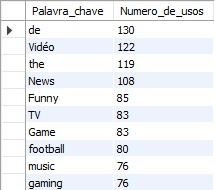
\includegraphics[width=0.4\textwidth]{consulta (3).jpg}
  \caption{Terceira consulta.}
\end{figure}

\subsection{Quarta consulta}

  Essa consulta apresenta cada país e o número de vezes que um canal sediado apareceu no \emph{Em Alta}. Consideramos como aparição cada ocorrência de canal sediado no país para cada vídeo seu no \emph{Em Alta} de um país em uma data.

\begin{code}
WITH
  Paises_em_alta AS
    (SELECT P.Codigo, CS.Canal_ID
         FROM Canal_Snapshot AS CS LEFT JOIN
        Pais AS P ON CS.Pais_Codigo = P.Codigo JOIN
          Video AS V USING (Canal_ID) JOIN
            Video_Snapshot AS VS ON V.ID = VS.Video_ID AND
                        CS.Data = VS.Data JOIN
              Trend AS T ON V.ID = T.Video_ID AND
                      VS.Data = T.Video_Snapshot_Data)
(SELECT Codigo AS Pais_sede, COUNT(Codigo) AS Numero_de_aparicoes
 FROM Paises_em_alta
 WHERE Codigo IS NOT NULL
 GROUP BY Codigo
 UNION
 SELECT NULL AS Pais_sede, COUNT(*) AS Numero_de_aparicoes
 FROM Paises_em_alta
 WHERE Codigo IS NULL)
ORDER BY Numero_de_aparicoes DESC;
\end{code}

\begin{figure}[H]
  \centering
  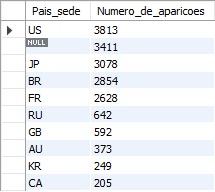
\includegraphics[width=0.4\textwidth]{consulta (4).jpg}
  \caption{Quarta consulta.}
\end{figure}

\subsection{Quinta consulta}

  Essa consulta exibe, em ordem decrescente de total de visualizações, os canais que mais tiveram visualizações em seus vídeos \emph{em alta} durante o período de coleta.

\begin{code}
WITH
  Video_mais_recente AS
    (SELECT V.ID, V.Canal_ID, VS.Numero_de_visualizacoes
         FROM Ultima_aparicao_video AS UAV JOIN
          Video AS V ON UAV.Video_ID = V.ID JOIN
            Video_Snapshot AS VS ON V.ID = VS.Video_ID AND
                        UAV.Ultima_data = VS.Data)
SELECT DISTINCT CS.Titulo AS Canal, VR.Total_de_visualizacoes
FROM (SELECT Canal_ID, SUM(Numero_de_visualizacoes) AS Total_de_visualizacoes
    FROM Video_mais_recente
      GROUP BY Canal_ID) AS VR JOIN
    Canal_Snapshot AS CS USING (Canal_ID)
ORDER BY VR.Total_de_visualizacoes DESC;
\end{code}

\begin{figure}[H]
  \centering
  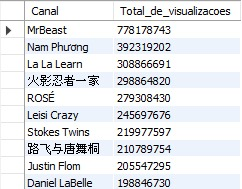
\includegraphics[width=0.4\textwidth]{consulta (5).jpg}
  \caption{Quinta consulta.}
\end{figure}


\chapter{Aplicação}

  A aplicação desenvolvida consiste de três componentes principais: o \emph{front-end} de HTML e \emph{JavaScript},
  o back-end escrito em \emph{Python}, e o servidor de banco de dados \emph{MySql}. O \emph{back-end} em \emph{Python}
  utiliza a biblioteca
  \emph{Flask} para estabelecer o servidor web, que serve inicialmente alguns arquivos estáticos e aguarda a escolha de uma
  consulta, cujos dados serão exibidos. A página inicial exibe um menu \emph{dropdown} em que se pode escolher entre cada
  uma das consultas possíveis à base de dados. Dependendo da consulta, o site então pergunta por dados adicionais. Por exemplo,
  qual canal consultar, ou sobre qual data se deseja obter informações. Para essas consultas, a \emph{query} padrão será
  completada através da definição de algumas \emph{user-defined variables}, para que seja específica aos parâmetros
  selecionados. Há então a consulta ao banco de dados através da biblioteca \emph{mysql} para \emph{Python}, e os dados
  serão retornados ao \emph{front-end} em arquivos HTML, populados por meio dos mecanismos de \emph{templates} do \emph{Flask}.
  Para gerar gráficos, o \emph{back-end} utiliza a biblioteca \emph{matplotlib}.

\chapter{Distribuição do trabalho}

   Inicialmente, os membros do grupo se reuniram para debater a modelagem conceitual para o tema proposto e, após diversos protótipos, Gustavo encontrou uma solução plausível para o modelagem sobre o tratamento da questão temporal dos nossos dados. 
   
   Em seguida, João Victor tratou da implementação do modelo conceitual no \nonport{BrModelo} e, junto de William Victor, realizaram a conversão para o modelo lógico e, em seguida, para o modelo físico. De forma quase assíncrona, Yuri e William Victor implementaram o programa que extraísse e tratasse os dados do \nonport{YouTube}.

   As consultas foram realizadas por William Victor.

   A respeito da implementação \nonport{Web}, em primeira instância, o grupo se reuniu para discutir os detalhes da aplicação e decidir pequenos detalhes. O uso da ferramenta \nonport{Flask} foi indicado por Gustavo, que, por sua vez, auxiliou Yuri na especificação da arquitetura da aplicação \nonport{Web}, incluindo as maneiras que a aplicação \nonport{front-end} se comunica com o \nonport{back-end} e, por sua vez, como o \nonport{back-end} se comunica com o banco de dados. Os códigos \nonport{html, css} e \nonport{javascript} foram escritos por Yuri.

    Sobre esse documento: os capítulos 1 e 2 foram escritos por William Victor e Yuri. Os capítulo 3 e 5 foram escritos por João Victor. O capítulo 4 foi escrito por Gustavo.

    Todos os capítulos desse documento sofreram atualizações conforme o desenvolvimento do trabalho. O confeccionamento, padronização e formatação do documento foi feito por João Victor.
    


\chapter{Considerações finais}

   \todo{Avaliar os resultados alcançados de acordo com os objetivos propostos.}

   Visto o objetivo inicial do projeto, concordamos que o resultado alcançado foi satisfatório. 
   
   Nenhum dos integrantes do grupo havia experiência prévia com bancos de dados ou desenvolvimento \nonport{Web} e, visto que conseguimos de forma satisfatória realizar o \nonport{data scraping}, inserir os dados coletados no SQL, manipular esses dados e, finalmente, realizar consultas dinâmicas ao banco de dados por meio da aplicação \nonport{Web}, concluímos que o resultado alcançado atendeu as expectativas.
